\PassOptionsToPackage{unicode=true}{hyperref} % options for packages loaded elsewhere
\PassOptionsToPackage{hyphens}{url}
%
\documentclass[]{article}
\usepackage{lmodern}
\usepackage{amssymb,amsmath}
\usepackage{ifxetex,ifluatex}
\usepackage{fixltx2e} % provides \textsubscript
\ifnum 0\ifxetex 1\fi\ifluatex 1\fi=0 % if pdftex
  \usepackage[T1]{fontenc}
  \usepackage[utf8]{inputenc}
  \usepackage{textcomp} % provides euro and other symbols
\else % if luatex or xelatex
  \usepackage{unicode-math}
  \defaultfontfeatures{Ligatures=TeX,Scale=MatchLowercase}
\fi
% use upquote if available, for straight quotes in verbatim environments
\IfFileExists{upquote.sty}{\usepackage{upquote}}{}
% use microtype if available
\IfFileExists{microtype.sty}{%
\usepackage[]{microtype}
\UseMicrotypeSet[protrusion]{basicmath} % disable protrusion for tt fonts
}{}
\IfFileExists{parskip.sty}{%
\usepackage{parskip}
}{% else
\setlength{\parindent}{0pt}
\setlength{\parskip}{6pt plus 2pt minus 1pt}
}
\usepackage{hyperref}
\hypersetup{
            pdftitle={Modelagem ARIMA e Análise de resíduos},
            pdfauthor={Lucas Resck e Lucas Moschen},
            pdfborder={0 0 0},
            breaklinks=true}
\urlstyle{same}  % don't use monospace font for urls
\usepackage{color}
\usepackage{fancyvrb}
\newcommand{\VerbBar}{|}
\newcommand{\VERB}{\Verb[commandchars=\\\{\}]}
\DefineVerbatimEnvironment{Highlighting}{Verbatim}{commandchars=\\\{\}}
% Add ',fontsize=\small' for more characters per line
\usepackage{framed}
\definecolor{shadecolor}{RGB}{248,248,248}
\newenvironment{Shaded}{\begin{snugshade}}{\end{snugshade}}
\newcommand{\AlertTok}[1]{\textcolor[rgb]{0.94,0.16,0.16}{#1}}
\newcommand{\AnnotationTok}[1]{\textcolor[rgb]{0.56,0.35,0.01}{\textbf{\textit{#1}}}}
\newcommand{\AttributeTok}[1]{\textcolor[rgb]{0.77,0.63,0.00}{#1}}
\newcommand{\BaseNTok}[1]{\textcolor[rgb]{0.00,0.00,0.81}{#1}}
\newcommand{\BuiltInTok}[1]{#1}
\newcommand{\CharTok}[1]{\textcolor[rgb]{0.31,0.60,0.02}{#1}}
\newcommand{\CommentTok}[1]{\textcolor[rgb]{0.56,0.35,0.01}{\textit{#1}}}
\newcommand{\CommentVarTok}[1]{\textcolor[rgb]{0.56,0.35,0.01}{\textbf{\textit{#1}}}}
\newcommand{\ConstantTok}[1]{\textcolor[rgb]{0.00,0.00,0.00}{#1}}
\newcommand{\ControlFlowTok}[1]{\textcolor[rgb]{0.13,0.29,0.53}{\textbf{#1}}}
\newcommand{\DataTypeTok}[1]{\textcolor[rgb]{0.13,0.29,0.53}{#1}}
\newcommand{\DecValTok}[1]{\textcolor[rgb]{0.00,0.00,0.81}{#1}}
\newcommand{\DocumentationTok}[1]{\textcolor[rgb]{0.56,0.35,0.01}{\textbf{\textit{#1}}}}
\newcommand{\ErrorTok}[1]{\textcolor[rgb]{0.64,0.00,0.00}{\textbf{#1}}}
\newcommand{\ExtensionTok}[1]{#1}
\newcommand{\FloatTok}[1]{\textcolor[rgb]{0.00,0.00,0.81}{#1}}
\newcommand{\FunctionTok}[1]{\textcolor[rgb]{0.00,0.00,0.00}{#1}}
\newcommand{\ImportTok}[1]{#1}
\newcommand{\InformationTok}[1]{\textcolor[rgb]{0.56,0.35,0.01}{\textbf{\textit{#1}}}}
\newcommand{\KeywordTok}[1]{\textcolor[rgb]{0.13,0.29,0.53}{\textbf{#1}}}
\newcommand{\NormalTok}[1]{#1}
\newcommand{\OperatorTok}[1]{\textcolor[rgb]{0.81,0.36,0.00}{\textbf{#1}}}
\newcommand{\OtherTok}[1]{\textcolor[rgb]{0.56,0.35,0.01}{#1}}
\newcommand{\PreprocessorTok}[1]{\textcolor[rgb]{0.56,0.35,0.01}{\textit{#1}}}
\newcommand{\RegionMarkerTok}[1]{#1}
\newcommand{\SpecialCharTok}[1]{\textcolor[rgb]{0.00,0.00,0.00}{#1}}
\newcommand{\SpecialStringTok}[1]{\textcolor[rgb]{0.31,0.60,0.02}{#1}}
\newcommand{\StringTok}[1]{\textcolor[rgb]{0.31,0.60,0.02}{#1}}
\newcommand{\VariableTok}[1]{\textcolor[rgb]{0.00,0.00,0.00}{#1}}
\newcommand{\VerbatimStringTok}[1]{\textcolor[rgb]{0.31,0.60,0.02}{#1}}
\newcommand{\WarningTok}[1]{\textcolor[rgb]{0.56,0.35,0.01}{\textbf{\textit{#1}}}}
\usepackage{longtable,booktabs}
% Fix footnotes in tables (requires footnote package)
\IfFileExists{footnote.sty}{\usepackage{footnote}\makesavenoteenv{longtable}}{}
\usepackage{graphicx,grffile}
\makeatletter
\def\maxwidth{\ifdim\Gin@nat@width>\linewidth\linewidth\else\Gin@nat@width\fi}
\def\maxheight{\ifdim\Gin@nat@height>\textheight\textheight\else\Gin@nat@height\fi}
\makeatother
% Scale images if necessary, so that they will not overflow the page
% margins by default, and it is still possible to overwrite the defaults
% using explicit options in \includegraphics[width, height, ...]{}
\setkeys{Gin}{width=\maxwidth,height=\maxheight,keepaspectratio}
\setlength{\emergencystretch}{3em}  % prevent overfull lines
\providecommand{\tightlist}{%
  \setlength{\itemsep}{0pt}\setlength{\parskip}{0pt}}
\setcounter{secnumdepth}{0}
% Redefines (sub)paragraphs to behave more like sections
\ifx\paragraph\undefined\else
\let\oldparagraph\paragraph
\renewcommand{\paragraph}[1]{\oldparagraph{#1}\mbox{}}
\fi
\ifx\subparagraph\undefined\else
\let\oldsubparagraph\subparagraph
\renewcommand{\subparagraph}[1]{\oldsubparagraph{#1}\mbox{}}
\fi

% set default figure placement to htbp
\makeatletter
\def\fps@figure{htbp}
\makeatother


\title{Modelagem ARIMA e Análise de resíduos}
\author{Lucas Resck e Lucas Moschen}
\date{\today}

\begin{document}
\maketitle

\hypertarget{muxe9todo-box-jenkins}{%
\section{Método Box-Jenkins}\label{muxe9todo-box-jenkins}}

\begin{enumerate}
\def\labelenumi{\arabic{enumi}.}
\setcounter{enumi}{-1}
\item
  Tranformação dos dados para estabilizar a variância.
\item
  Identificação
\end{enumerate}

1.1 Checar a estacionaridade e diferencial \(d\) vezes;

1.2 Visualizar autocorrelação e autocorrelação parcial dos dados;

1.3 Comparar informações AIC, BIC e AICc e selectionar \(p\) e \(q\).

\begin{enumerate}
\def\labelenumi{\arabic{enumi}.}
\setcounter{enumi}{1}
\tightlist
\item
  Estimação
\end{enumerate}

2.1 Estimar os valores de \(\phi\) e \(\theta\) do modelo através de
máxima verossimilhança.

\begin{enumerate}
\def\labelenumi{\arabic{enumi}.}
\setcounter{enumi}{2}
\tightlist
\item
  Diagnóstico
\end{enumerate}

3.1 Visualizar os resíduos do fitting;

3.2 Plotar histograma, autocorrelação e autocorrelação parcial dos
resíduos;

3.3 Testes de estacionaridade e de normalidade.

\hypertarget{assassinato-de-mulheres}{%
\section{Assassinato de mulheres}\label{assassinato-de-mulheres}}

Primeiro, vamos visualizar a série anual. Peecebemos uma clara
tendência, com crescimento acentuado ao longo das décadas de 1960 e
1970, bem como um decréscimo após os anos de 1990.

\includegraphics{arima_modelling_files/figure-latex/unnamed-chunk-1-1.pdf}

\hypertarget{transformauxe7uxe3o-box-cox}{%
\subsection{Transformação Box-Cox}\label{transformauxe7uxe3o-box-cox}}

Dada a nossa série, é importante que visualizemos a variância ao longo
dela. Visualmente ela aparenta não ter variância constante, dado que no
início da série, ela aparenta ser menor. Para isso vamos calcular a
transformação ótima de Box-Cox.

A transformação de Box-Cox é a seguinte, se \(\{y_t\}\) for uma série
temporal,

\[
y_t^{(\lambda)} = \begin{cases} \frac{y_t^{\lambda} - 1}{\lambda}, \text{ se } \lambda \neq 0\\ \log(y_t),  \text{ se } \lambda = 0\end{cases}
\]

A escolha de \(\lambda\) ótimo utiliza o método de Guerrero, que escolhe
\(\lambda\) que minimize o coeficiente de variação
(\(c_v = \frac{\sigma}{\mu}\)) para subséries de \(y_t\). A seguir
podemos conferir o resultado da transformação.

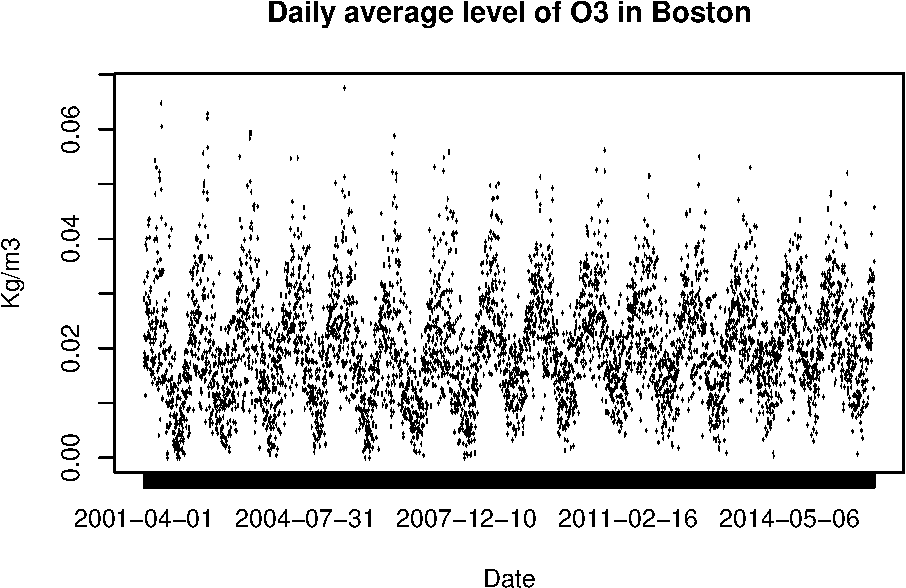
\includegraphics{arima_modelling_files/figure-latex/unnamed-chunk-2-1.pdf}

\hypertarget{identificauxe7uxe3o}{%
\subsection{Identificação}\label{identificauxe7uxe3o}}

\hypertarget{teste-de-estacionaridade-adf}{%
\subsubsection{Teste de Estacionaridade
ADF}\label{teste-de-estacionaridade-adf}}

\begin{Shaded}
\begin{Highlighting}[]
\KeywordTok{adf.test}\NormalTok{(bcwmurders)}
\end{Highlighting}
\end{Shaded}

\begin{verbatim}
## Warning in adf.test(bcwmurders): p-value greater than printed p-value
\end{verbatim}

\begin{verbatim}
## 
##  Augmented Dickey-Fuller Test
## 
## data:  bcwmurders
## Dickey-Fuller = -0.027131, Lag order = 3, p-value = 0.99
## alternative hypothesis: stationary
\end{verbatim}

Como \(\text{p-valor} \ge 0.05\), inferimos a não estacioanridade.

\hypertarget{diferenciando}{%
\subsubsection{Diferenciando}\label{diferenciando}}

\includegraphics{arima_modelling_files/figure-latex/unnamed-chunk-4-1.pdf}

\begin{Shaded}
\begin{Highlighting}[]
\KeywordTok{adf.test}\NormalTok{(dwmurders)}
\end{Highlighting}
\end{Shaded}

\begin{verbatim}
## 
##  Augmented Dickey-Fuller Test
## 
## data:  dwmurders
## Dickey-Fuller = -3.6064, Lag order = 3, p-value = 0.04084
## alternative hypothesis: stationary
\end{verbatim}

\includegraphics{arima_modelling_files/figure-latex/unnamed-chunk-6-1.pdf}

É inconclusivo, piriri, pororo.

\begin{longtable}[]{@{}rrrrr@{}}
\toprule
p & q & AIC & BIC & AICC\tabularnewline
\midrule
\endhead
0 & 0 & -157.8102 & -153.8322 & -157.5749\tabularnewline
0 & 1 & -156.0378 & -150.0709 & -155.5578\tabularnewline
0 & 2 & -159.8467 & -151.8907 & -159.0303\tabularnewline
0 & 3 & -158.0477 & -148.1028 & -156.7977\tabularnewline
1 & 0 & -156.1778 & -150.2109 & -155.6978\tabularnewline
1 & 1 & -156.6976 & -148.7416 & -155.8813\tabularnewline
1 & 2 & -157.9735 & -148.0285 & -156.7235\tabularnewline
1 & 3 & -156.1456 & -144.2117 & -154.3583\tabularnewline
2 & 0 & -159.4687 & -151.5127 & -158.6523\tabularnewline
2 & 1 & -157.6280 & -147.6831 & -156.3780\tabularnewline
2 & 2 & -158.9166 & -146.9827 & -157.1294\tabularnewline
2 & 3 & -157.2561 & -143.3332 & -154.8213\tabularnewline
3 & 0 & -157.5952 & -147.6503 & -156.3452\tabularnewline
3 & 1 & -155.4728 & -143.5389 & -153.6856\tabularnewline
3 & 2 & -157.4078 & -143.4849 & -154.9730\tabularnewline
3 & 3 & -155.9103 & -139.9984 & -152.7103\tabularnewline
\bottomrule
\end{longtable}

Baseado no AIC e AICc, o modelo é (0,2). O BIC também caracteriza (0,2)
como um bom modelo.

\hypertarget{estimauxe7uxe3o}{%
\subsection{Estimação}\label{estimauxe7uxe3o}}

\begin{Shaded}
\begin{Highlighting}[]
\NormalTok{model <-}\StringTok{ }\KeywordTok{Arima}\NormalTok{(wmurders, }\DataTypeTok{order =} \KeywordTok{c}\NormalTok{(}\DecValTok{0}\NormalTok{,}\DecValTok{1}\NormalTok{,}\DecValTok{2}\NormalTok{), }\DataTypeTok{lambda =} \StringTok{"auto"}\NormalTok{)}
\KeywordTok{summary}\NormalTok{(model)}
\end{Highlighting}
\end{Shaded}

\begin{verbatim}
## Series: wmurders 
## ARIMA(0,1,2) 
## Box Cox transformation: lambda= -0.09529835 
## 
## Coefficients:
##           ma1     ma2
##       -0.0907  0.3770
## s.e.   0.1283  0.1723
## 
## sigma^2 estimated as 0.002701:  log likelihood=83.92
## AIC=-161.85   AICc=-161.37   BIC=-155.88
## 
## Training set error measures:
##                        ME      RMSE      MAE        MPE     MAPE      MASE
## Training set -0.001070576 0.1996771 0.154647 -0.1341953 4.430353 0.9510067
##                    ACF1
## Training set 0.03120906
\end{verbatim}

\hypertarget{diagnuxf3stico}{%
\subsection{Diagnóstico}\label{diagnuxf3stico}}

\begin{Shaded}
\begin{Highlighting}[]
\KeywordTok{checkresiduals}\NormalTok{(model)}
\end{Highlighting}
\end{Shaded}

\includegraphics{arima_modelling_files/figure-latex/unnamed-chunk-10-1.pdf}

\begin{verbatim}
## 
##  Ljung-Box test
## 
## data:  Residuals from ARIMA(0,1,2)
## Q* = 8.6023, df = 8, p-value = 0.3769
## 
## Model df: 2.   Total lags used: 10
\end{verbatim}

\begin{Shaded}
\begin{Highlighting}[]
\KeywordTok{jarque.bera.test}\NormalTok{(model}\OperatorTok{$}\NormalTok{residuals)}
\end{Highlighting}
\end{Shaded}

\begin{verbatim}
## 
##  Jarque Bera Test
## 
## data:  model$residuals
## X-squared = 0.13536, df = 2, p-value = 0.9346
\end{verbatim}

Não rejeitamos nenhuma das hipóteses. Estamos satisfeitos.

\hypertarget{projeuxe7uxe3o}{%
\subsection{Projeção}\label{projeuxe7uxe3o}}

\begin{Shaded}
\begin{Highlighting}[]
\KeywordTok{forecast}\NormalTok{(model, }\DataTypeTok{h =} \DecValTok{3}\NormalTok{) }\OperatorTok\StringTok{ }\KeywordTok{autoplot}\NormalTok{()}
\end{Highlighting}
\end{Shaded}

\includegraphics{arima_modelling_files/figure-latex/unnamed-chunk-11-1.pdf}

\hypertarget{uso-de-cartuxe3o-de-duxe9bito}{%
\section{Uso de cartão de débito}\label{uso-de-cartuxe3o-de-duxe9bito}}

Primeiro, vamos visualizar a série. Percebemos uma sutil sazonalidade,
aparentemente anual, além de uma clara tendência.

\includegraphics{arima_modelling_files/figure-latex/unnamed-chunk-12-1.pdf}

\hypertarget{transformauxe7uxe3o-box-cox-1}{%
\subsection{Transformação Box-Cox}\label{transformauxe7uxe3o-box-cox-1}}

Pelo gráfico, parece que teremos que fazer alguma transformação de
estabilidade da variância. Para isso, vamos utilizar a transformação
Box-Cox.

\includegraphics{arima_modelling_files/figure-latex/unnamed-chunk-13-1.pdf}

\hypertarget{identificauxe7uxe3o-1}{%
\subsection{Identificação}\label{identificauxe7uxe3o-1}}

Agora, com a variância da série estabilizada, podemos fazer o teste de
estacionaridade. Observe que o teste ADF possui possibilidade de
tendência. Assim

\hypertarget{teste-de-estacionaridade-adf-1}{%
\subsubsection{Teste de Estacionaridade
ADF}\label{teste-de-estacionaridade-adf-1}}

\begin{Shaded}
\begin{Highlighting}[]
\KeywordTok{adf.test}\NormalTok{(bcdebitcards)}
\end{Highlighting}
\end{Shaded}

\begin{verbatim}
## 
##  Augmented Dickey-Fuller Test
## 
## data:  bcdebitcards
## Dickey-Fuller = -3.0873, Lag order = 5, p-value = 0.1227
## alternative hypothesis: stationary
\end{verbatim}

Como \(\text{p-valor} \ge 0.05\), não podemos rejeitar a hipótese nula
de que a série é não estacionária. Portanto, vamos usar a primeira
diferenciação.

\hypertarget{diferenciando-1}{%
\subsubsection{Diferenciando}\label{diferenciando-1}}

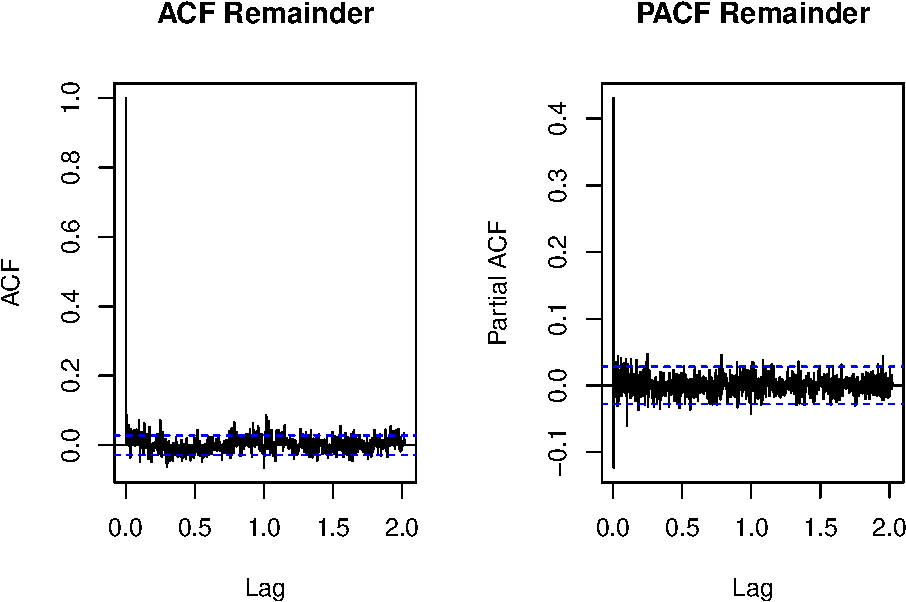
\includegraphics{arima_modelling_files/figure-latex/unnamed-chunk-15-1.pdf}

\begin{Shaded}
\begin{Highlighting}[]
\KeywordTok{adf.test}\NormalTok{(ddebitcards)}
\end{Highlighting}
\end{Shaded}

\begin{verbatim}
## Warning in adf.test(ddebitcards): p-value smaller than printed p-value
\end{verbatim}

\begin{verbatim}
## 
##  Augmented Dickey-Fuller Test
## 
## data:  ddebitcards
## Dickey-Fuller = -8.3838, Lag order = 5, p-value = 0.01
## alternative hypothesis: stationary
\end{verbatim}

Assim, podemos rejeitar a hipótese nula, o que suporta a ideia de que a
série é estacionária. Vamos considerar

\hypertarget{acf-e-pacf}{%
\subsubsection{ACF e PACF}\label{acf-e-pacf}}

\includegraphics{arima_modelling_files/figure-latex/unnamed-chunk-17-1.pdf}

Percebemos dois fatores bem destacados: uma grande correlação quando o
\(\text{Lag} = 12\), o que indica que existe uma sazonalidade anual; e
que a PACF decresce exponencialmente, enquanto a ACF morre após
\(\text{Lag} = 1\), o que nos levaria a um modelo MA(1). Antes disso,
vamos fazer uma diferenciação a cada 12 meses.

\includegraphics{arima_modelling_files/figure-latex/unnamed-chunk-18-1.pdf}

\begin{verbatim}
## Warning in adf.test(ddebitcards): p-value smaller than printed p-value
\end{verbatim}

\begin{verbatim}
## 
##  Augmented Dickey-Fuller Test
## 
## data:  ddebitcards
## Dickey-Fuller = -5.4939, Lag order = 5, p-value = 0.01
## alternative hypothesis: stationary
\end{verbatim}

Observe que ainda temos uma série estacionária. Vejamos a ACF e PACF
novamente:

\includegraphics{arima_modelling_files/figure-latex/unnamed-chunk-20-1.pdf}

O pico diminuiu consideravelmente. Agora, sim, vamos considerar os
critérios de informação para identificar o modelo.

\hypertarget{crituxe9rios-de-informauxe7uxe3o}{%
\subsubsection{Critérios de
Informação}\label{crituxe9rios-de-informauxe7uxe3o}}

\begin{longtable}[]{@{}rrrrr@{}}
\toprule
p & q & AIC & BIC & AICC\tabularnewline
\midrule
\endhead
0 & 0 & -277.1636 & -271.1291 & -277.0825\tabularnewline
0 & 1 & -339.0449 & -329.9930 & -338.8816\tabularnewline
0 & 2 & -339.0065 & -326.9374 & -338.7326\tabularnewline
0 & 3 & -342.2090 & -327.1226 & -341.7952\tabularnewline
0 & 4 & -342.0094 & -323.9057 & -341.4261\tabularnewline
0 & 5 & -345.7949 & -324.6739 & -345.0116\tabularnewline
1 & 0 & -311.2501 & -302.1983 & -311.0869\tabularnewline
1 & 1 & -337.9786 & -325.9095 & -337.7046\tabularnewline
1 & 2 & -338.9584 & -323.8720 & -338.5446\tabularnewline
1 & 3 & -341.1438 & -323.0401 & -340.5604\tabularnewline
1 & 4 & -342.3731 & -321.2522 & -341.5899\tabularnewline
1 & 5 & -343.8243 & -319.6860 & -342.8102\tabularnewline
2 & 0 & -343.2455 & -331.1764 & -342.9716\tabularnewline
2 & 1 & -343.9712 & -328.8848 & -343.5574\tabularnewline
2 & 2 & -342.0010 & -323.8973 & -341.4177\tabularnewline
2 & 3 & -340.0692 & -318.9482 & -339.2859\tabularnewline
2 & 4 & -345.1572 & -321.0189 & -344.1431\tabularnewline
2 & 5 & -354.2751 & -327.1196 & -352.9985\tabularnewline
3 & 0 & -343.8279 & -328.7415 & -343.4141\tabularnewline
3 & 1 & -341.9907 & -323.8870 & -341.4073\tabularnewline
3 & 2 & -343.4891 & -322.3682 & -342.7059\tabularnewline
3 & 3 & -341.8366 & -317.6984 & -340.8226\tabularnewline
3 & 4 & -339.8344 & -312.6788 & -338.5578\tabularnewline
3 & 5 & -350.4613 & -320.2885 & -348.8899\tabularnewline
4 & 0 & -341.9974 & -323.8937 & -341.4140\tabularnewline
4 & 1 & -340.0049 & -318.8839 & -339.2217\tabularnewline
4 & 2 & -341.7904 & -317.6522 & -340.7763\tabularnewline
4 & 3 & -339.8401 & -312.6846 & -338.5635\tabularnewline
4 & 4 & -350.3646 & -320.1918 & -348.7932\tabularnewline
4 & 5 & -353.3164 & -320.1263 & -351.4171\tabularnewline
5 & 0 & -340.0364 & -318.9154 & -339.2531\tabularnewline
5 & 1 & -338.0020 & -313.8638 & -336.9879\tabularnewline
5 & 2 & -341.2724 & -314.1169 & -339.9958\tabularnewline
5 & 3 & -344.0011 & -313.8283 & -342.4297\tabularnewline
5 & 4 & -345.4699 & -312.2798 & -343.5706\tabularnewline
5 & 5 & -349.3232 & -313.1158 & -347.0623\tabularnewline
\bottomrule
\end{longtable}

Baseado no AIC e AICc, o modelo é ARMA(2,5). Baseado no BIC escolhemos
um modelo bem mis simples, ARMA(2,0). Vou seguir com o modelo com mais
parâmetros.

\hypertarget{estimauxe7uxe3o-1}{%
\subsection{Estimação}\label{estimauxe7uxe3o-1}}

Estimamos os parâmetros do modelo, considerando uma diferenciação
sazonal.

\begin{Shaded}
\begin{Highlighting}[]
\NormalTok{model <-}\StringTok{ }\KeywordTok{Arima}\NormalTok{(debitcards, }\DataTypeTok{order =} \KeywordTok{c}\NormalTok{(}\DecValTok{2}\NormalTok{,}\DecValTok{1}\NormalTok{,}\DecValTok{5}\NormalTok{), }\DataTypeTok{seasonal =} \KeywordTok{c}\NormalTok{(}\DecValTok{0}\NormalTok{,}\DecValTok{1}\NormalTok{,}\DecValTok{0}\NormalTok{), }\DataTypeTok{lambda =} \StringTok{"auto"}\NormalTok{)}
\KeywordTok{summary}\NormalTok{(model)}
\end{Highlighting}
\end{Shaded}

\begin{verbatim}
## Series: debitcards 
## ARIMA(2,1,5)(0,1,0)[12] 
## Box Cox transformation: lambda= 0.09078485 
## 
## Coefficients:
##          ar1      ar2      ma1     ma2      ma3      ma4     ma5
##       1.1563  -0.7891  -2.0007  1.9044  -0.3988  -0.5641  0.4453
## s.e.  0.0746   0.0632   0.1042  0.2100   0.2417   0.1881  0.0951
## 
## sigma^2 estimated as 0.004985:  log likelihood=186.12
## AIC=-356.23   AICc=-355.22   BIC=-332.09
## 
## Training set error measures:
##                       ME      RMSE       MAE        MPE     MAPE      MASE
## Training set -0.03028165 0.8570868 0.6404297 -0.2238406 3.952716 0.4998296
##                   ACF1
## Training set 0.0607404
\end{verbatim}

\hypertarget{diagnuxf3stico-1}{%
\subsection{Diagnóstico}\label{diagnuxf3stico-1}}

Aqui podemos conferir os resíduos. É importante detacar a aparência
normal dos resíduos, o que é interessante. Porém a ACF ainda apresenta
picos, o mais incomodativo é do período 12.

O test Ljung-Box coorrobora esse fato, rejeitando a hipótese nula de que
os coeficientes de correlação são iguais. Já Jarque Bera não rejeita a
normalidade, como esperávamos.

\begin{Shaded}
\begin{Highlighting}[]
\KeywordTok{checkresiduals}\NormalTok{(model)}
\end{Highlighting}
\end{Shaded}

\includegraphics{arima_modelling_files/figure-latex/unnamed-chunk-24-1.pdf}

\begin{verbatim}
## 
##  Ljung-Box test
## 
## data:  Residuals from ARIMA(2,1,5)(0,1,0)[12]
## Q* = 42.875, df = 17, p-value = 0.0005007
## 
## Model df: 7.   Total lags used: 24
\end{verbatim}

\begin{Shaded}
\begin{Highlighting}[]
\KeywordTok{jarque.bera.test}\NormalTok{(model}\OperatorTok{$}\NormalTok{residuals)}
\end{Highlighting}
\end{Shaded}

\begin{verbatim}
## 
##  Jarque Bera Test
## 
## data:  model$residuals
## X-squared = 2.6451, df = 2, p-value = 0.2664
\end{verbatim}

O persistente pico pode ser um indicativo de que a série sazonal precise
de coeficientes ARMA. Em particular, poderíamos colocar ARMA sazonal.
Isso fica para as próximas análises.

\hypertarget{projeuxe7uxe3o-1}{%
\subsection{Projeção}\label{projeuxe7uxe3o-1}}

Agora vamos conferir as projeções três passos a frente.

\begin{Shaded}
\begin{Highlighting}[]
\KeywordTok{forecast}\NormalTok{(model, }\DataTypeTok{h =} \DecValTok{3}\NormalTok{) }\OperatorTok\StringTok{ }\KeywordTok{autoplot}\NormalTok{()}
\end{Highlighting}
\end{Shaded}

\includegraphics{arima_modelling_files/figure-latex/unnamed-chunk-25-1.pdf}

\hypertarget{comer-fora-na-austruxe1lia}{%
\section{Comer fora na Austrália}\label{comer-fora-na-austruxe1lia}}

Primeiro, vamos visualizar a série.

\includegraphics{arima_modelling_files/figure-latex/unnamed-chunk-26-1.pdf}

\end{document}
